\section{Results}
\label{cha::rsr::results}
To evaluate RSR we use a generic implementation of A* and discuss performance 
in terms of search time speedup. That is, the relative improvement to the average 
time A* needs to solve an instance when running on a pruned  vs. unpruned grid.
For example, a speedup of 2.0 is twice as fast (higher is better).
Note that on approximately 2\% of all instances the start and goal are located
in the same rectangle and RSR computes the optimal solution without
search.  We exclude these instances from our results even though RSR solves
them in constant time. Their exclusion makes for a clearer comparison between
RSR and contemporary approaches from the pathfinding literature.

\par 
\begin{figure*}[t]
\begin{center}
   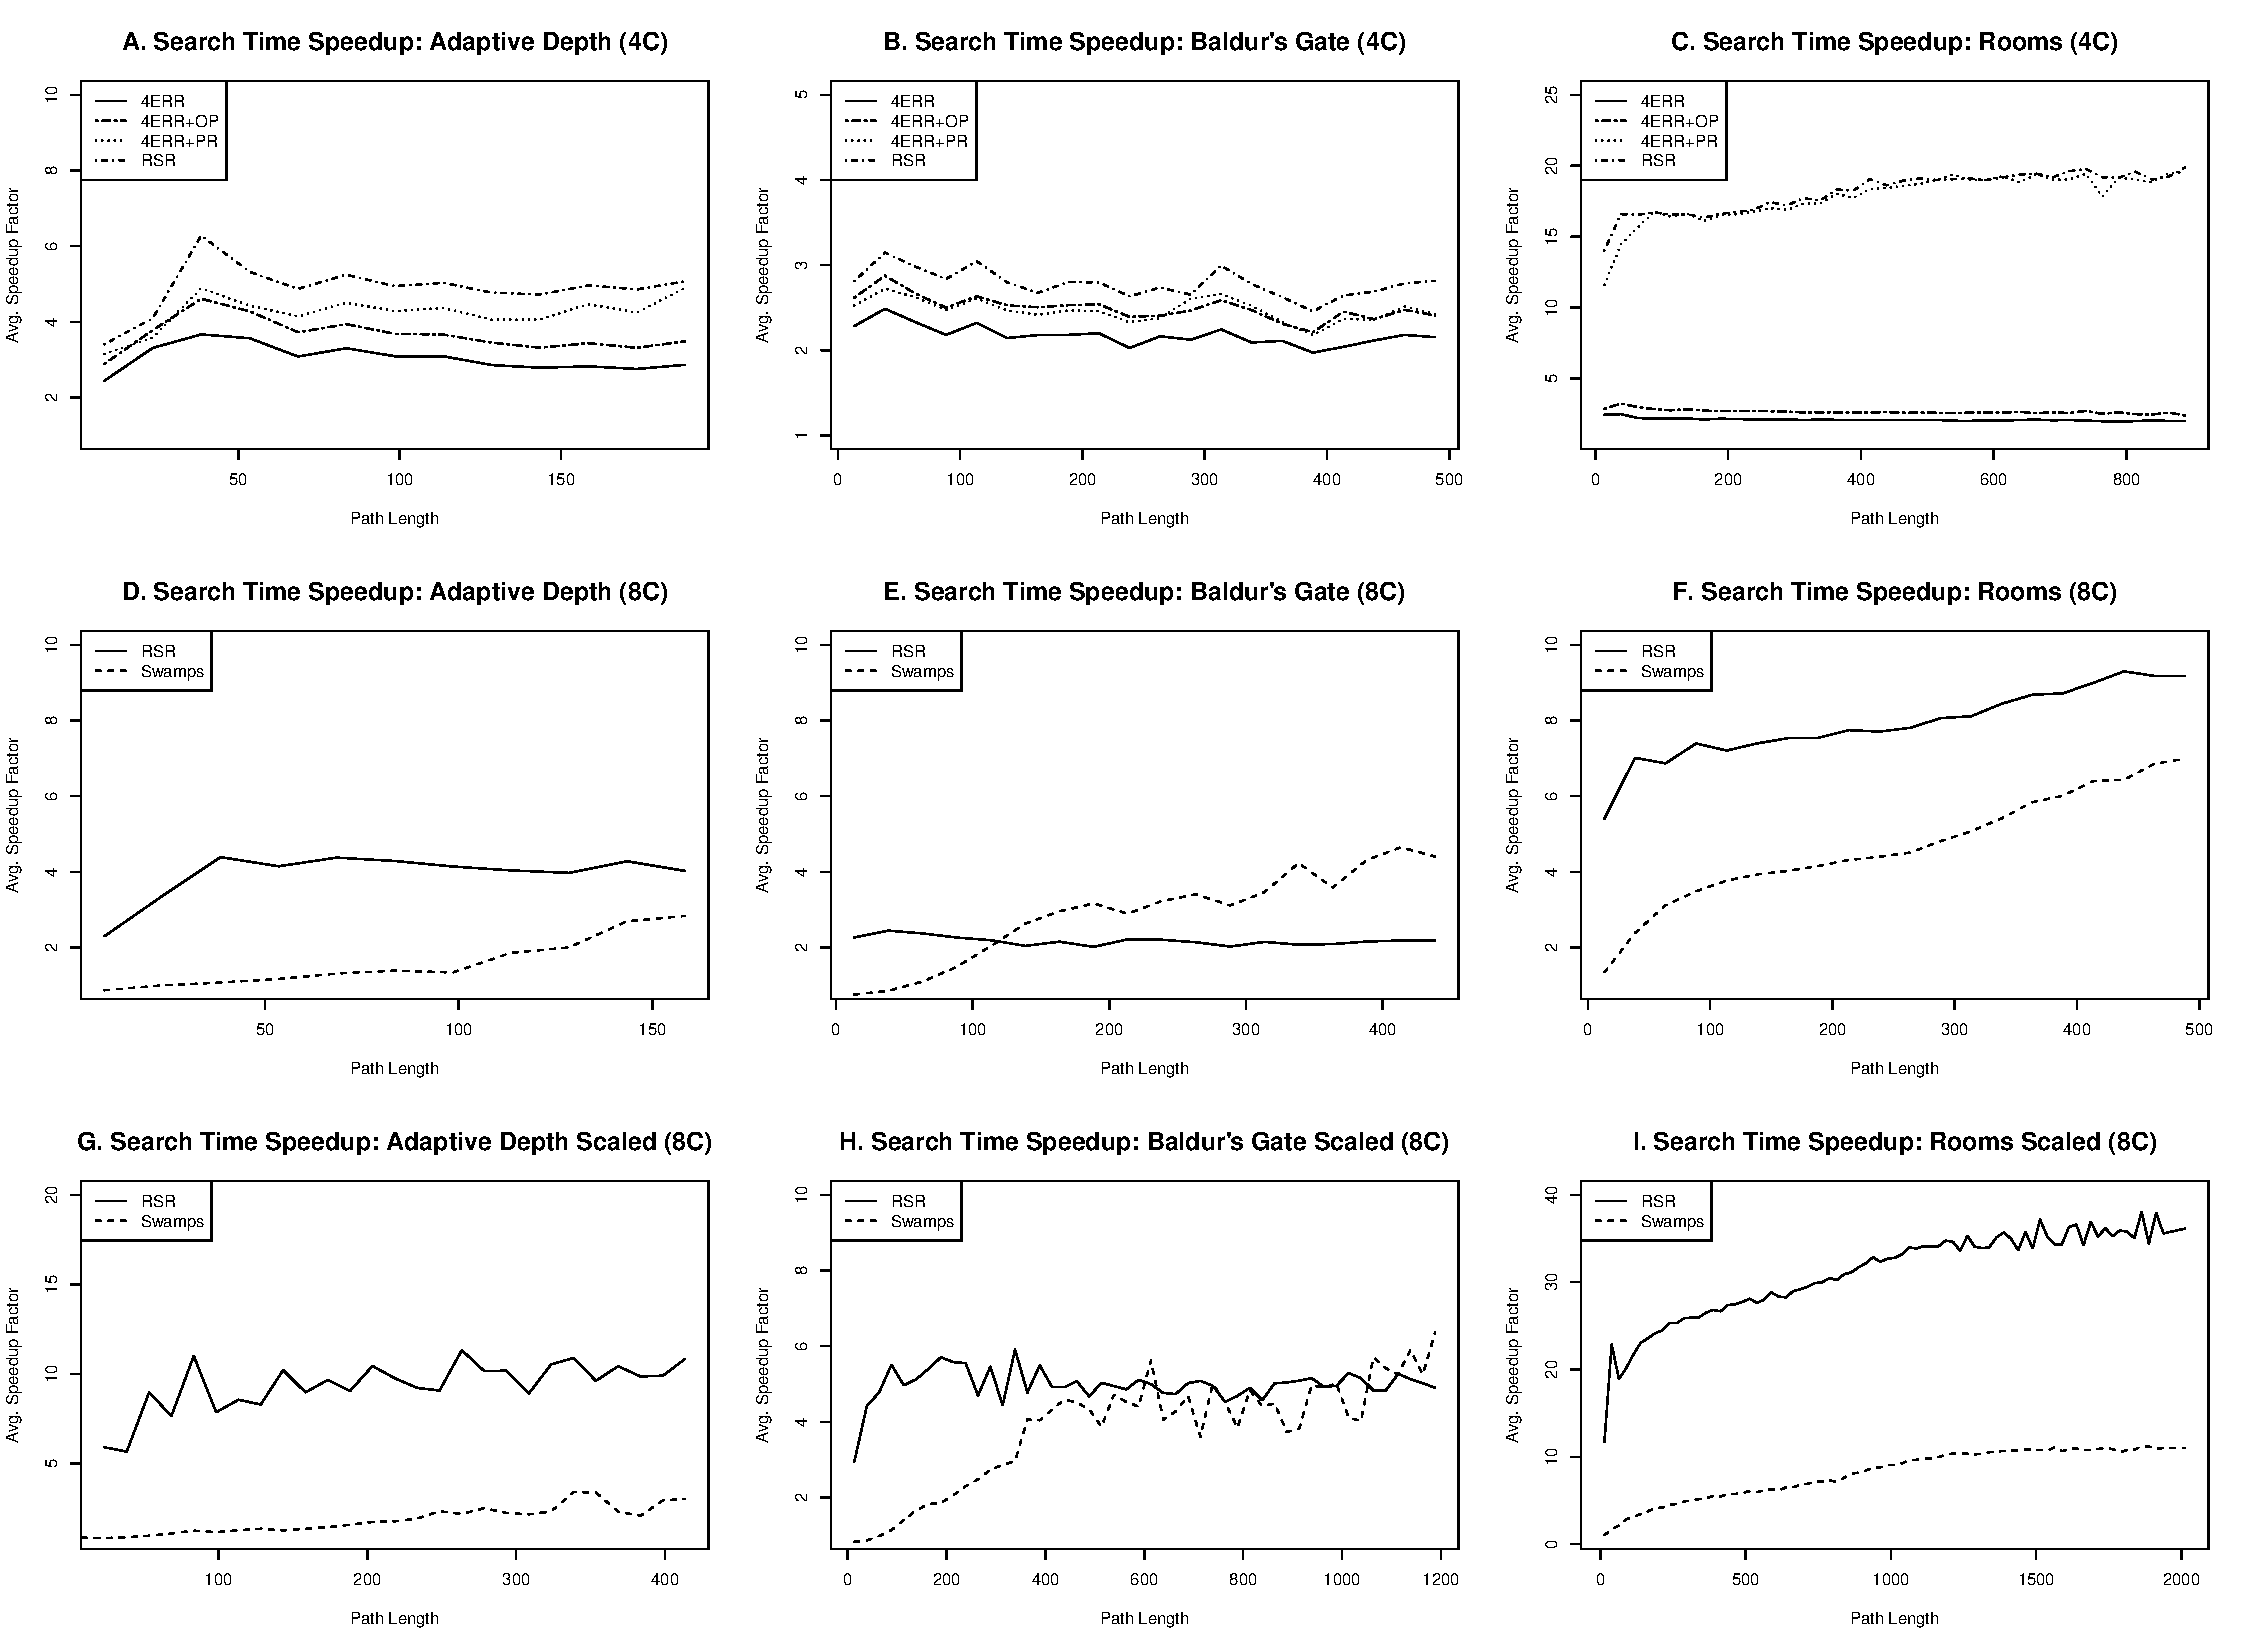
\includegraphics[width=0.97\columnwidth, trim = 10mm 10mm 10mm 0mm]{chapter_rsr/diagrams/speedup.pdf}
\end{center}
\caption[Search time speedup: RSR]
{\small 
Average A* speedup on each of our three benchmarks. 
Results are given in terms of relative improvement to A* search time (i.e. speedup).}
\label{fig::rsr::speedup}
\end{figure*}


\textbf{Pre-processing Times: } 
Table 1 presents a summary of average pre-processing times for
each of our three (non-scaled) benchmarks. We also give the average number of
nodes and edges as an indication of map size.
We notice that RSR takes very little time to pre-process all input maps. 
We did not encounter any that took longer than a second, and most required 
significantly less than that. 
%An interesting implication from this result is that RSR appears well suited to
%pathfinding in dynamic environments as outlined in Section \ref{sec:memory}.

\input chapter_rsr/table_preproc

\subsection{4-Connected Grid Maps}
We begin with an evaluation of RSR on 4-connected grid maps. 
For comparison, we will develop several intermediate variations
of the algorithm. These allow us to assess the individual impact
of each of the ideas described in this chapter.
4ERR (4-Connected Empty Rectangular Rooms) refers to the simple
symmetry breaking approach from Section~\ref{cha::rsr::symm4c}.
4ERR+OP is the combination of 4ERR with online node pruning only and 
4ERR+PR is the combination of 4ERR with perimeter reduction only.
Figure \ref{fig::rsr::speedup} (A to C) presents the main result of the
chapter.
\par
Note that RSR (== ERR+OP+PR) shows a convincing 
speed improvement over 4ERR and all its variants across all input maps.
This allows us to conclude that that RSR is the better choice on 4-connected maps.
When analysing the impact of each enhancement, we note that 4ERR+PR yields the
biggest improvement on all three benchmarks, speeding up A* by up to 20 times.
4ERR+OP compares well with 4ERR+PR on both Adaptive Depth and
Baldur's Gate but is of little benefit on Rooms where perimeter pruning has
already reduced the branching factor.
\par
The large performance variation from one benchmark to another can be attributed
to how effectively we can decompose the map. A good decomposition forms large
rectangles with few perimeter nodes after pruning. This is the case for Rooms.
A poor decomposition builds small rectangles with many transitionary perimeter 
nodes that cannot be pruned. This is the case for Baldur's Gate. 

\subsection{Comparison to Swamps:}
Next, we compare and contrast the performance of RSR with the Swamps
algorithm~\citep{pochter10}.  To evaluate Swamps we used the authors' source
code, including their own implementation of A*.  We then ran all experiments
using their recommended running parameters: a swamp seed radius of 6 and ``no
change limit'' of 2.
Figure \ref{fig::rsr::speedup} (D to F) gives search time speedup results for both RSR
and Swamps running on the 8-connected variants of our three benchmark problem
sets. 
On Adaptive Depth and Rooms, where the terrain can be naturally decomposed into
rectangles, RSR achieves higher speedups and is shown consistently better than Swamps. 
On Baldur's Gate, where the 45-degree orientation of maps reduces the effectiveness
of rectangle decomposition, Swamps-based pruning is more effective. 
\par
Next, we scaled every map in each benchmark by a factor of 3 and randomly
generated a new set of 100 problem instances per map.  Scaling has the effect of
producing larger open areas and allows us to measure the impact of this variable
on search time speedup.  We present our findings in  Figure \ref{fig::rsr::speedup} (G
to I).  We observe that while the maximum speedup achieved by both algorithms
has increased, the gain for Swamps is very small while RSR shows dramatic
improvement.  Infact, if we limit our attention to problems of similar length to
those seen on the original maps we notice that the performance of Swamps
actually decreases.
\par
The observed performance characteristics are not unexpected: Swamps prune out
\textit{areas that can be avoided} without introducing a detour while rectangle-based
symmetry reduction allows for a faster exploration of \textit{areas that need to be
searched}.  Since it appears that the two algorithms are orthogonal, a natural
extension of this work would be to combine the two: first, apply 4(or 8)ERR+PR
(as appropriate) to a grid in order to eliminate as many interior nodes as
possible; then, apply a Swamps-based decomposition to the resultant graph.

\input chapter_rsr/table_portals

\subsection{Comparison to Portal Heuristic:}
We now compare RSR with PH-e -- the enhanced variant of the recent 
Portal Heuristic algorithm \citep{goldenberg10}.
Although we did not have access to a working implementation of this method we
will discuss its performance vs. RSR based on published results obtained by the
original authors. As in \citep{goldenberg10} we focus on the 4-connected variants 
of the Baldur's Gate and Rooms benchmarks.
Table 2 summarises the main result.
\par
PH-e performs well when it can decompose the map into areas of similar size with
few transitionary nodes connecting them.
RSR performs well when it can decompose the map into large rectangles with few
perimeter nodes.
On Rooms, both decomposition approaches are highly effective. 
On Baldur's Gate both are comparatively less effective.
Notice however that PH-e requires up to 7 times more memory than RSR to achieve
similar results.
PH-e narrows the scope of search to a corridor of nodes inside which the
optimal path can be found. This means that, like Swamps, PH-e and RSR
are entirely orthogonal and two can be easily combined. 
One possible combination involves using PH-e to more accurately guide search
on a map pruned by RSR. Another possibility involves using symmetry
elimination to speed up speed up pathfinding between successive pairs of
portals during PH-e's refinement phase.
